% This must be in the first 5 lines to tell arXiv to use pdfLaTeX, which is strongly recommended.
\pdfoutput=1
% In particular, the hyperref package requires pdfLaTeX in order to break URLs across lines.

\documentclass[11pt]{article}

% Remove the "review" option to generate the final version.
\usepackage[]{acl2020}

% Standard package includes
\usepackage{times}
\usepackage{latexsym}

% For proper rendering and hyphenation of words containing Latin characters (including in bib files)
\usepackage[T1]{fontenc}
% For Vietnamese characters
% \usepackage[T5]{fontenc}
% See https://www.latex-project.org/help/documentation/encguide.pdf for other character sets

% This assumes your files are encoded as UTF8
\usepackage[utf8]{inputenc}

% This is not strictly necessary, and may be commented out,
% but it will improve the layout of the manuscript,
% and will typically save some space.
\usepackage{microtype}

%% added by pia:
\usepackage{amsmath,amssymb,mathtools} % Math
\usepackage{url}
\usepackage{multirow} 
\usepackage{booktabs}
\usepackage{natbib}

% If the title and author information does not fit in the area allocated, uncomment the following
%
%\setlength\titlebox{<dim>}
%
% and set <dim> to something 5cm or larger.

\title{Machine Learning for Named Entity Recognition and Classification\\ Report, Theoretical Component, and NERC-Research Preparation}

% Author information can be set in various styles:
% For several authors from the same institution:
% \author{Author 1 \and ... \and Author n \\
%         Address line \\ ... \\ Address line}
% if the names do not fit well on one line use
%         Author 1 \\ {\bf Author 2} \\ ... \\ {\bf Author n} \\
% For authors from different institutions:
% \author{Author 1 \\ Address line \\  ... \\ Address line
%         \And  ... \And
%         Author n \\ Address line \\ ... \\ Address line}
% To start a seperate ``row'' of authors use \AND, as in
% \author{Author 1 \\ Address line \\  ... \\ Address line
%         \AND
%         Author 2 \\ Address line \\ ... \\ Address line \And
%         Author 3 \\ Address line \\ ... \\ Address line}

\author{Vera Langeberg}

\begin{document}



\maketitle
\begin{abstract}
    Fill in a short abstract for your final submission.

\end{abstract}

%The final report has a strict maximum of 6 pages (12 columns)

\textcolor{magenta}{We recommend aiming for a report of around 6. This does not include acknowledgements or references (they may appear on page 7 and later if needed). You can use appendices if you want to share more details. Below, we provide length indications per section. Please try to stick to them, but don't worry about receiving a lower grade if you don't quite manage. They are supposed to help you and prevent you from doing extra work.}

\section{Introduction}

\textcolor{magenta}{Length: ±  1/2 - max 1 column for Introduction}


Write a short introduction to your approach for the final submission. The introduction should include:

\begin{itemize}
    \item A brief description of the task (not detailed)
    \item An outline of the ML approaches included in the report
    \item A brief summary of your results
\end{itemize}

\begin{itemize}
    \item[] \textit{Assignment 3}
\end{itemize}



\section{Task and Data}

\textcolor{magenta}{Length: ± 1.5-2 columns for Task and Data.}


\subsection{Task}



\begin{itemize}
    \item[]
          The exact task of NER given the CoNLL dataset is to identify and classify named entity spans in text into predefined categories.
          These categories are: locations (LOC), organizations (ORG), miscellaneous names (MISC), and persons (PER).
          Named entities are typically spans of text that can consist of one or more tokens.
          However, to simplify the task and transform it from span identification into a token classification problem, the BIO (Beginning, Inside, Outside) tagging scheme is used.
          This scheme allows us to represent multi-token entity spans while still classifying individual tokens.
          Before them, there is a B- or I- to indicate whether it is the beginning or inside of an entity.
          The O label indicates that the token is outside of any named entity.
          This results in the following labels present in the dataset:
          "{'B-LOC', 'I-ORG', 'I-MISC', 'B-MISC', 'O', 'B-ORG', 'I-PER', 'I-LOC', 'B-PER'}"

          For example, in the phrase "Vera Langeberg lives in Amsterdam":

          The span "Vera Langeberg" is a person entity:
          "Vera" would be labeled as "B-PER" (beginning of person span)
          "Langeberg" would be labeled as "I-PER" (inside of person span)
          "lives" and "in" would be labeled as "O" (outside any entity span)
          The span "Amsterdam" is a location entity:
          "Amsterdam" would be labeled as "B-LOC" (beginning of location span)
          This approach allows the NER system to identify both single-token and multi-token named entity spans while performing token-level classification, effectively bridging the gap between span identification and token classification.

    \item[] \textit{Assignment 2} Update if necessary
    \item[] \textit{Assignment 3} Update if necessary
\end{itemize}

\subsection{Dataset and Distribution}



\begin{itemize}
    \item[]
          The dataset used in this project is the CoNLL-2003 dataset, which is specifically designed for Named Entity Recognition (NER) tasks \cite{sang2003introductionconll2003sharedtask}.
          The CoNLL format consists of for columns separated by spaces.
          Empty rows indicate sentence boundaries.
          The columns are as follows:
          \begin{itemize}
              \item Word or token
              \item Part-of-speech tag
              \item Chunk tag
              \item Named Entity tag
          \end{itemize} \cite{sang2003introductionconll2003sharedtask}[p.2]

          For example, in the line:
          \begin{verbatim}
LONDON	NNP	B-NP	B-LOC
\end{verbatim}
          "London" is the token, "NNP" is the part-of-speech tag (indicating a proper noun), "B-NP" is the chunk tag (indicating that it is the beginning of a noun phrase), and "B-LOC" is the named entity tag (indicating that it is the beginning of a location entity).
          The total number of tokens in the CoNLL training set is 203621.
          As can be seen in \ref{fig:label_distribution}, the majority of the tokens are labeled with the O tag, indicating that they are outside of any named entity.
          The most frequent named entity label is B-LOC (7140), followed by B-PER (6600) and B-ORG (6321), as shown in \ref{fig:label_distribution_without_O}.
          The least represented named entity label is I-MISC together with I-LOC. They only have 1155 and 1157 occurrences respectively in the training set.
          \begin{figure}[htbp]
              \centering
              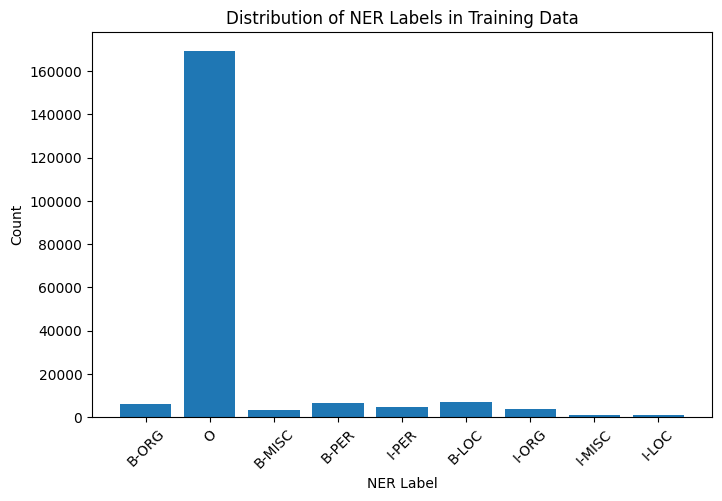
\includegraphics[width=0.7\linewidth]{figures/label_distribution.png}
              \caption{Label distribution in the CoNLL training set.}
              \label{fig:label_distribution}
          \end{figure}

          \begin{figure}[htbp]
              \centering
              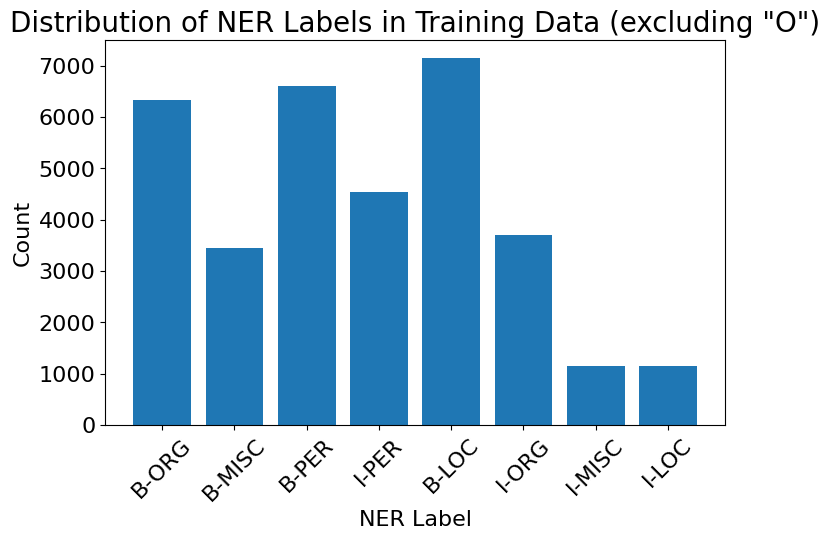
\includegraphics[width=0.7\linewidth]{figures/label_distribution_without_o.png}
              \caption{Label distribution in the CoNLL training set (excluding "O").}
              \label{fig:label_distribution_without_O}
          \end{figure}

          In \ref{fig:most_common_words_per_label_no_IOB}, the most common words for location, persons, organizations and miscellaneous names are shown.
          Here the IOB tags have been removed for clarity.
          For location, "u.s" is most common, "cup" is most common for miscellaneous names,"clinton" for persons and "of" for organizations.

    \item[] \textit{Assignment 2} update if necessary
    \item[] \textit{Assignment 3} update if necessary
\end{itemize}



\subsection{Preprocessing}

\begin{itemize}
    \item[] The only preprocessing that was done for the initial dataset analysis was lowercasing the tokens for the most frequent words per category.
          This was only done to collect the most frequent words, to avoid having the same word in different cases.
          Since, the case of the token is an important feature for NER, the original casing was kept for the model training.
          No stopword removal or stemming/lemmatization was applied. Also no special characters were removed yet.
          This might be done in later assignments.

    \item[] \textit{Assignment 2} update (if applicable)
    \item[] \textit{Assignment 3} update (if applicable)
\end{itemize}



\subsection{Evaluation Metrics}

\begin{itemize}
    \item[]
          This paper will focus on token-level evaluation for the assignments.
          This means, that the BIO tags will be taken into account when calculating the metrics and have to match exactly.
          If only a partial match is made (so either wrong BIO tag, or wrong NE label), it will be considered incorrect.
    \item[] \textit{Assignment 2 and 3}: Update if necessary
\end{itemize}


\section{Models and Features}

\textcolor{magenta}{Length: ± 2 columns for Models and Features.}

\subsection{Models}

\begin{itemize}
    \item[] \textit{Assignment 1} The model used in the basic system is a Logistic Regression classifier from the sklearn library.
          Despite its name, it is mostly used for classification tasks. It has a linear model as its core that uses the sigmoid function to output probabilities for each class.
          The model coefficients represent the importance of each feature for each class.
          The model was trained using the default parameters from sklearn on the training set.

    \item[]\textit{Assignment 2} Alternative Methods (SVM, NB)
    \item[]\textit{Assignment 3} More advanced models (fine-tuning BERT, CRF for ReMA students only)
\end{itemize}


\subsection{Features}

\begin{itemize}
    \item[] \textit{Assignment 1} Feature exploration
          In this paper the features that were used in the basic system are:
          \begin{itemize}
              \item Token itself: The actual word provides crucial semantic information. Certain words are more likely to be part of specific entity types (e.g., "Inc." often indicates an organization).
              \item POS tags: Part-of-speech information helps identify potential named entities. For instance, proper nouns (NNP) are often good candidates for named entities.
              \item Capitalization: In English, this is a strong indicator for named entities, as proper nouns are typically capitalized. It helps distinguish between common nouns and potential named entities, though it can be less reliable at the beginning of sentences.
          \end{itemize}
          These features provide complementary information that aids in identifying and classifying named entities.
          The token itself carries semantic content, POS tags offer syntactic clues, and capitalization provides orthographic hints that are particularly useful for recognizing proper nouns.

          The distribution of all these features can be found in the \ref{sec:linguistic_features}.
    \item[] \textit{Assignment 2} More features
    \item[] \textit{Assignment 3} More advanced features
\end{itemize}



\section{Experiments and Results}

\textcolor{magenta}{Length: ± 3 columns (including figures and tables) for Experiments and Results. Additional material can be provided in the Appendix.}

\subsection{Evaluation}

\begin{itemize}
    \item [] \textit{Assignment 1}: first results
          The first results of the basic system on the development set are shown in figure \ref{fig:log_results} and the confusion matrix \ref{fig:confusion_matrix_log}.
          \begin{figure}[htbp]
              \centering
              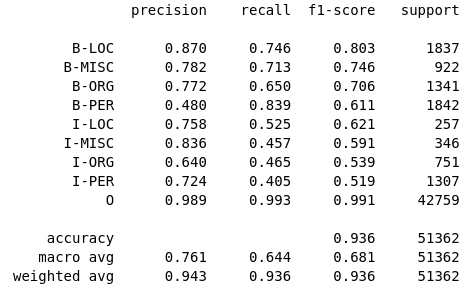
\includegraphics[width=0.7\linewidth]{figures/results_log.png}
              \caption{Results of the Logistic Regression model on the development set.}
              \label{fig:log_results}
          \end{figure}
          \begin{figure}[htbp]
              \centering
              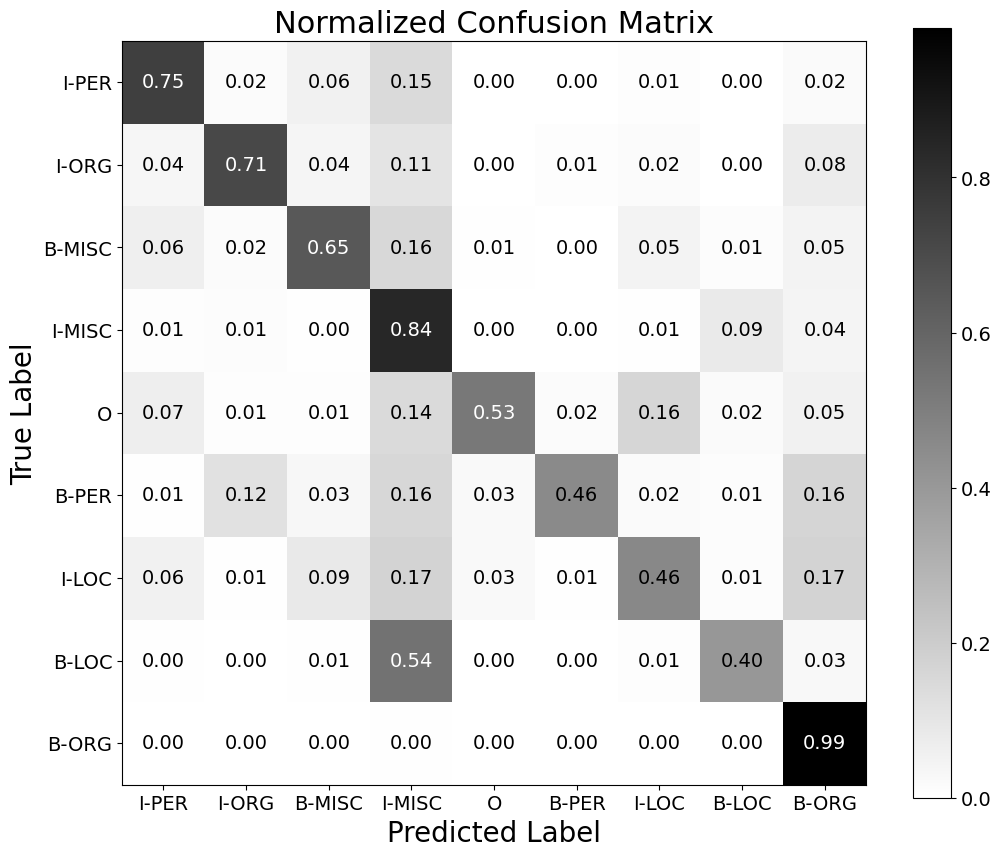
\includegraphics[width=0.7\linewidth]{figures/confusion_matrix_log.png}
              \caption{Confusion matrix of the Logistic Regression model on the development set.}
              \label{fig:confusion_matrix_log}
          \end{figure}
          As can be seen, the model performs best on the B-LOC label with a 0.99 accuracy.
          The model struggles the most with the B-ORG label, with an accuracy of 0.40.
          The largest confusion happens between B-ORG that gets predicted as B-PER a lot.
          The macro precision is 0.761 and the macro recall is 0.644. The accuracy is with 0.936 quite high already.

    \item [] \textit{Assignment 2}: update
    \item [] \textit{Assignment 3}: update
\end{itemize}

\subsection{Feature Ablation}

\begin{itemize}
    \item [] \textit{Assignment 3}: feature ablation for one system \textcolor{magenta}{Note: if you decide after your feature ablation that you would like to discuss this before the Evaluation, you may move this subsection.}
\end{itemize}


\section{Error Analysis}

\textcolor{magenta}{Length: ± 1.5-2 columns for Error Analysis.}

\begin{itemize}
    \item [] \textit{Assignment 3}: beyond the confusion matrix
\end{itemize}


\section{Discussion}

\textcolor{magenta}{Length: ± 1 column for Discussion and Conclusion together.}

\begin{itemize}
    \item [] \textit{Assignment 3}
\end{itemize}

\section{Conclusion}

\begin{itemize}
    \item [] \textit{Assignment 3}
\end{itemize}






\section*{Acknowledgements}



% Entries for the entire Anthology, followed by custom entries
\bibliography{references}

\clearpage


\appendix

\section*{Theoretical Component}

\subsection*{Assignment 1 - What is Machine learning?}

My answer on the question "What is Machine learning" starts with explaining the intuition behind it.
Machine learning is about machines learning, but this sounds still very silly and unclear.
Therefore, lets first dive into the machines part.
People should not think about machines like the first typewriter, or motor engines, or even your normal kitchen blender.
We should also not think about the computers or calculators that run simple algorithms.
Algorithms are mostly strictly defined, like the ones embedded in your regular calculators.
These machines do not learn, they just follow a set of rules that are already defined.
This is not machine learning, it is following a recipe.
If the recipe is bad, you will get a burned cake. If you don't adjust the oven temperature next time, the cake will burn over and over again.
The machines we are looking at are different.
They can learn from data, identify patterns, and make decisions based on that data
To get back to our cake, this means that after one time burning the cake, it will lower the temperature next time, or even adjust the baking time.
It can be undercooked that time, but it will learn from that as well, and adjust again.
This learning from data and identifying patterns is the essence of machine learning.

When looking at it in a bit more formal way, machine learning is a subset of artificial intelligence (AI) that focuses on the development of algorithms and statistical models that enable computers to perform specific tasks without explicit instructions.
Instead of being explicitly programmed to perform a task, machine learning algorithms use data to learn patterns and make predictions or decisions.
This is done by training the algorithms on large datasets, allowing them to learn from the data and improve their performance over time.
Machine learning can be categorized into three main types: supervised learning, unsupervised learning, and reinforcement learning.
In supervised learning, the algorithm is trained on labeled data, where the input data is paired with the correct output.
The algorithm learns to map the input to the output and can make predictions on new, unseen data.
In unsupervised learning, the algorithm is trained on unlabeled data and must find patterns and relationships in the data on its own.
Reinforcement learning involves training an agent to make decisions in an environment by rewarding or punishing it based on its actions.
Key in the development of good machine learning algorithms are examples, features, and labels.
Examples are the individual data points that the algorithm learns from.
Features are the attributes or characteristics of the examples that are used to make predictions.
Labels are the correct outputs or categories that the algorithm is trying to predict.
To test the performance of machine learning algorithms, evaluation metrics such as accuracy, precision, recall, and F1-score are used.
The evaluation is typically done on a separate dataset that was not used during training, known as the test set.
A golden testset is a testset that is carefully curated and annotated by experts to ensure high quality and reliability.

\subsection*{Assignment 2}


\subsection*{Assignment 3}



\clearpage

\section*{Time spent}\label{app.time}

\begin{table}[!htb]
    \centering
    \small{
        \begin{tabular}{p{1cm}p{3cm}p{1cm}}
            \toprule
            Week  & Task                                                   & Time       \\
            \midrule
            1     & Understand the assignment and getting everything setup & 30 minutes \\
            1     & Watch the videos of module 1                           & 2 hours    \\
            1     & Finish 2.1 about understanding NER and CoNLL           & 1.5 hours  \\
            1     & Work on 2.2.1 further exploration of the data          & 1 hour     \\
            1     & Work on 2.2.2 feature hypothesis                       & 1 hour     \\
            1     & Started with 3.1, description of precision, recall etc & 0.5 hour   \\
            1     & Did all the week 2 tasks for assignment 1              & 2 hours    \\
            1     & Incorporated the feedback for assignment 1             & 1.5 hours  \\
            \midrule
            Total & 10h                                                                 \\

            \bottomrule
        \end{tabular}
        \caption{Time overview. \label{time} }}
\end{table}

\section{Example Appendix}
\label{sec:appendix}

This is an appendix. You can include additional analyses and tables here (e.g.\ samples you analyzed for your error analysis).

\clearpage

\section*{NERC-research preparation}
\subsection*{2.1.1 - NER given the CoNLL dataset}
In this course we will use the CoNLL-2003 dataset, which is specifically designed for Named Entity Recognition (NER) tasks \cite{sang2003introductionconll2003sharedtask}.
The exact task of NER given the CoNLL dataset is to identify and classify named entities in text into predefined categories.
These categories are: locations (LOC), organizations (ORG), miscellaneous names (MISC), and persons (PER).
Before them, there is a B- or I- to indicate whether it is the beginning or inside of an entity.
The O label indicates that the token is outside of any named entity.
This results in the following labels present in the dataset:
"{'B-LOC', 'I-ORG', 'I-MISC', 'B-MISC', 'O', 'B-ORG', 'I-PER', 'I-LOC', 'B-PER'}"

The conventions that are followed in this dataset is IOB tagging scheme.
This means that when a named entity consists of multiple tokens, the first token is labeled with a B- (beginning) and the subsequent tokens with I- (inside).
For example, in the entity "New York City", "New" would be labeled as B-LOC, "York" as I-LOC, and "City" as I-LOC.
There is consistency in the labeling, meaning that if a token is labeled as I-ORG, it must be preceded by either B-ORG or another I-ORG.

Punctuation marks are represented as separate tokens and are labeled with the O tag, indicating that they are outside of any named entity.
\subsection*{2.2.1 - How does CoNLL work?}
The CoNLL format consists of for columns separated by spaces.
Empty rows indicate sentence boundaries.
The columns are as follows:
\begin{itemize}
    \item Word or token
    \item Part-of-speech tag
    \item Chunk tag
    \item Named Entity tag
\end{itemize} \cite{sang2003introductionconll2003sharedtask}[p.2]

For example, in the line:
\begin{verbatim}
    LONDON	NNP	B-NP	B-LOC
\end{verbatim}
"London" is the token, "NNP" is the part-of-speech tag (indicating a proper noun), "B-NP" is the chunk tag (indicating that it is the beginning of a noun phrase), and "B-LOC" is the named entity tag (indicating that it is the beginning of a location entity).

\subsection*{2.2.1 - Distribution of the labels}
To investigate the distribution of the labels in the CoNLL dataset, I wrote a small piece of code that extracts the labels from the dataset and counts their frequency.
The total number of tokens in the training set is 203621.
The results show that the majority of the tokens are labeled with the O tag, indicating that they are outside of any named entity.
This was what I expected, as not all tokens in a text are part of named entities.
When looking at the named entity labels, I found that the most frequent named entity label is B-LOC (7140), followed by B-PER (6600) and B-ORG (6321).
The least represented named entity label is I-MISC together with I-LOC. They only have 1155 and 1157 occurrences respectively in the training set.


\subsection*{2.2.2 - Hypothesis about linguistic features that might help NER}\label{sec:linguistic_features}
I hypothesize that the following linguistic and orthographic features might help improve NER performance:
- Part-of-speech tags: Certain parts of speech, such as proper nouns (NNP), are more likely to be named entities. Including POS tags as features can help the model identify potential named entities.
- Capitalization: Named entities often start with capital letters. Including a feature that indicates whether a token is capitalized can help the model distinguish named entities from common nouns.
- Contextual words: The words surrounding a token can provide important context for identifying named entities. "the" or "an" or "a" is very common before a named entity.
Including features that capture these patterns can help the model recognize named entities.

To test if these features have influence on the NER performance, I wrote some code in the notebook.
Starting with the POS tags. I extracted the POS tags from the dataset and counted their frequency.
The results show that the most common POS tags in the CoNLL training set are NNP \ref{fig:pos_distribution}.
\begin{figure}
    \centering
    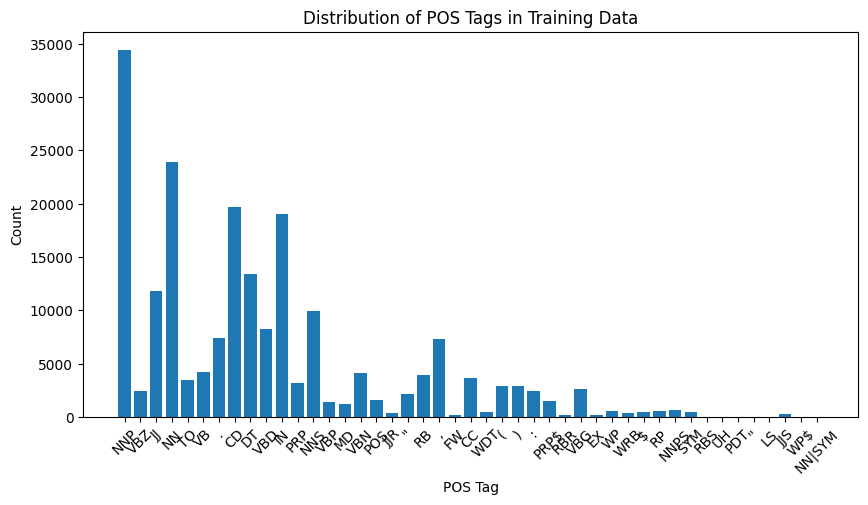
\includegraphics[width=0.7\linewidth]{figures/POS.png}
    \caption{Distribution of POS tags in the CoNLL training set.}
    \label{fig:pos_distribution}
\end{figure}
Next, I looked at the capitalization feature. I counted the number of capitalized tokens versus non-capitalized tokens.
The results show that a significant (about 25\%) portion of the tokens in the CoNLL training set are capitalized \ref{fig:capitalization_distribution}.
\begin{figure}
    \centering
    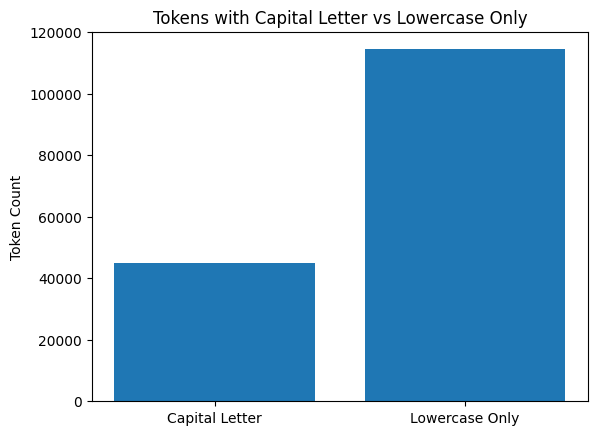
\includegraphics[width=0.7\linewidth]{figures/capitalized.png}
    \caption{Capitalization distribution in the CoNLL training set.}
    \label{fig:capitalization_distribution}
\end{figure}
Finally, I analyzed the contextual words preceding named entities.
I extracted the tokens that appear before named entities and counted their frequency.
The results show that certain tokens, such as "the", "of", and "in", are more common before named entities \ref{fig:tokens_before_NE} and \ref{fig:ne_preceding_tokens}.
This didn't correspond exactly with my hypothesis, as I expected more articles like "a" and "an" to be present.
\begin{figure}
    \centering
    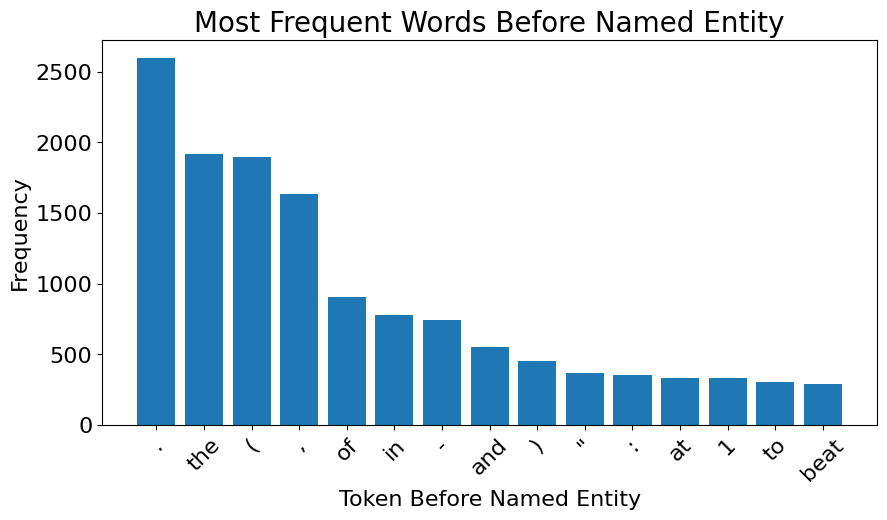
\includegraphics[width=0.7\linewidth]{figures/tokens_before_NE.png}
    \caption{Top 15 most common tokens before named entities in the CoNLL training set.}
    \label{fig:tokens_before_NE}
\end{figure}
\begin{figure}
    \centering
    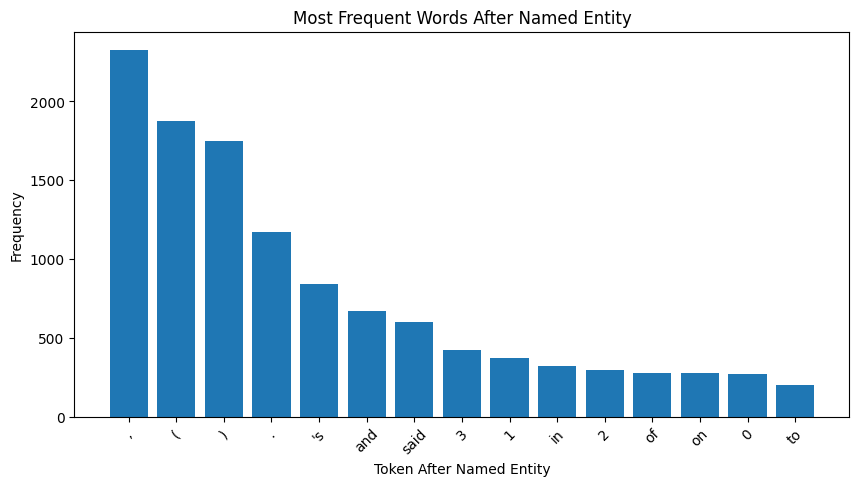
\includegraphics[width=0.7\linewidth]{figures/NE_preciding_tokes.png}
    \caption{Top 15 most common tokens preceding named entities in the CoNLL training set.}
    \label{fig:ne_preceding_tokens}
\end{figure}

Next, I explored the most common words per category.
\begin{figure}
    \centering
    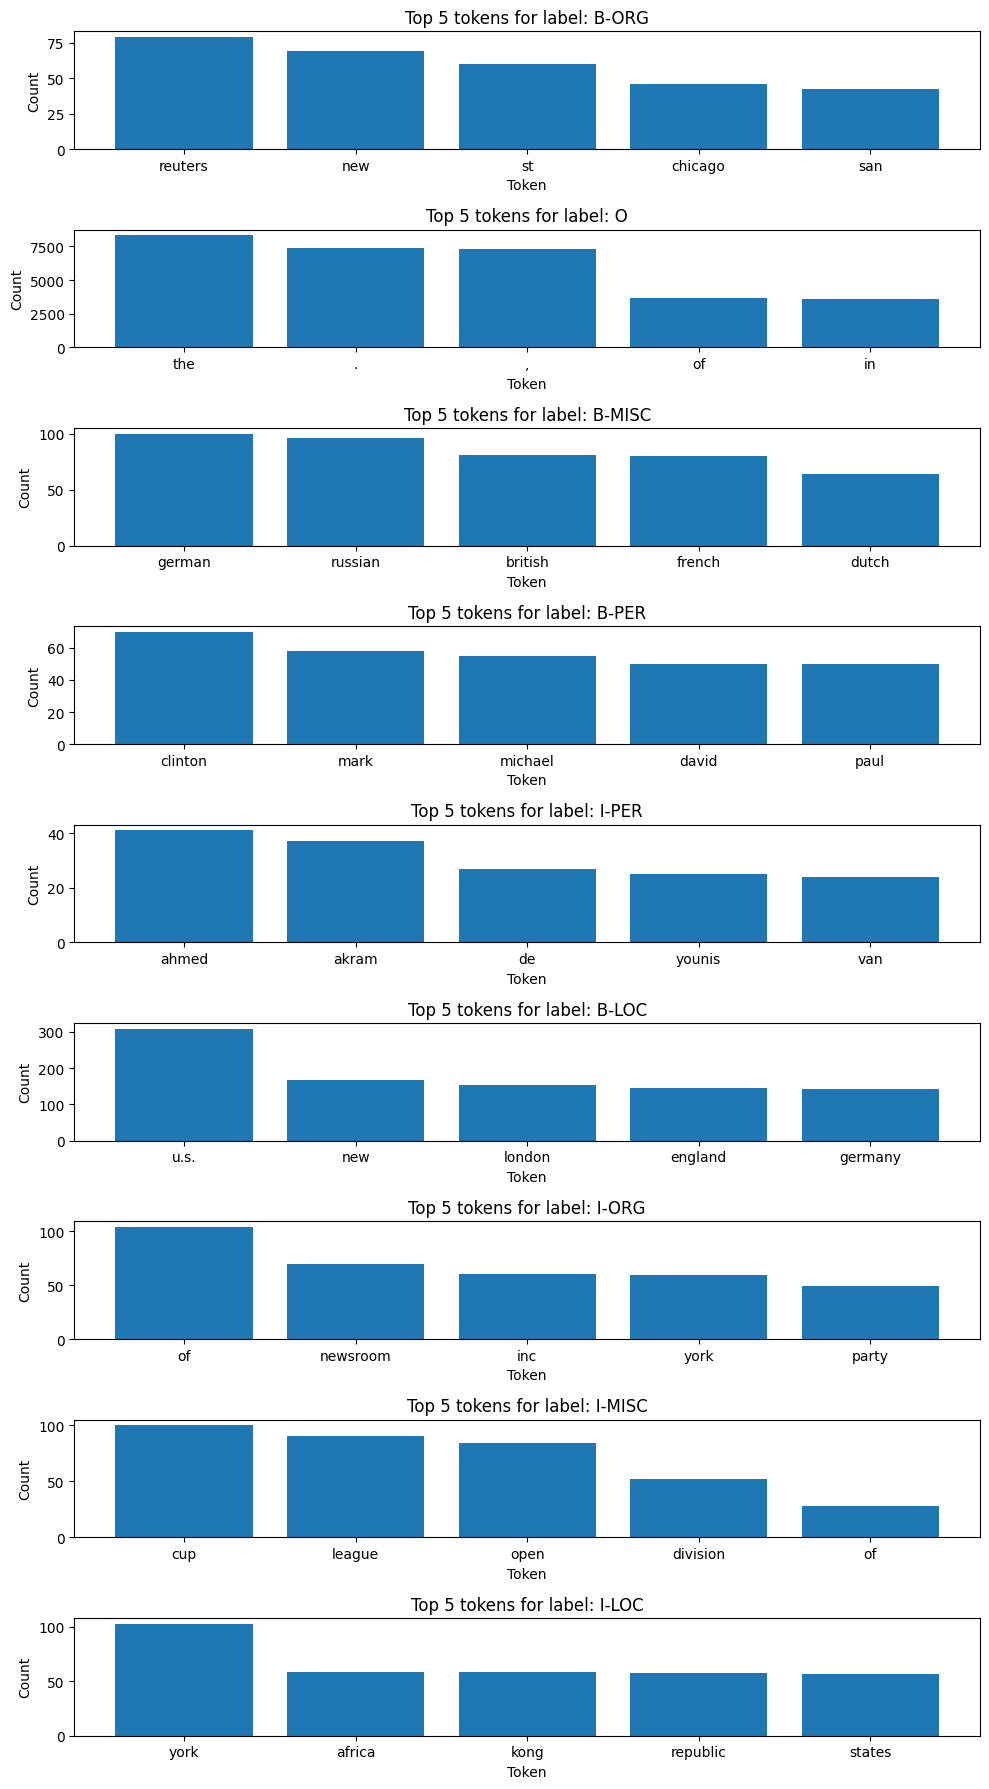
\includegraphics[width=0.7\linewidth]{figures/word_freq_with_IOB.png}
    \caption{Most common words per named entity label in the CoNLL training set.}
    \label{fig:most_common_words_per_label_with_IOB}
\end{figure}
Since the figure \ref{fig:most_common_words_per_label_with_IOB} is a bit hard to read, I created a new graph without the IOB tags.
This graph shows the most common words for location, persons, organizations and miscellaneous names. \ref{fig:most_common_words_per_label_no_IOB}.
For location, "u.s" is most common, "cup" is most common for miscellaneous names,"clinton" for persons and "of" for organizations.
\begin{figure}
    \centering
    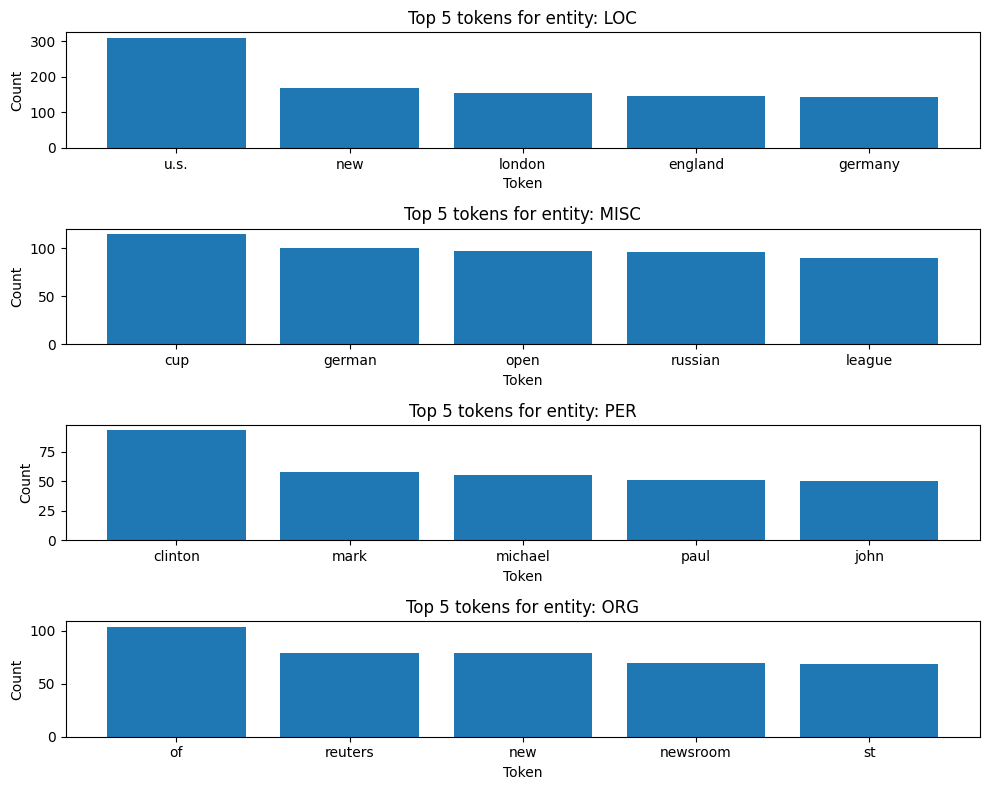
\includegraphics[width=0.7\linewidth]{figures/word_freq_without_IOB.png}
    \caption{Most common words per named entity label (without IOB) in the CoNLL training set.}
    \label{fig:most_common_words_per_label_no_IOB}
\end{figure}



\subsection*{3. 1. Confusion matrix}
In this section I discuss the terms precision, recall and F-score in my own words.
The precision of a model is the proportion of true predictions compared to all instances that got the true label.
So how much that got filtered out, was actually correct.
The recall of a model is the proportion of true predictions compared to all instances that actually have that label.
How much of what should have been filtered out, was actually filtered out.
The F-score is the harmonic mean of precision and recall, providing a single metric to evaluate the model's performance.
This takes both precision and recall into account, and balances them.
A scenario where high precision is most important is your spam email filter.
We all hate when we missed an important email because it got filtered as spam.
When you would have a high precision, everything that is in the spam folder is actually spam.
A scenario where high recall is most important is in medical dermatology diagnosis.
It is worse to miss a cancer diagnosis (false negative) than to have a false alarm (false positive).
These are the classic examples that were also used in previous courses I followed.

\subsection*{3.2. Code for confusion matrix and metrics}
I already implemented the code to calculate recall, precision and F1-score.
There is also a way to plot the confusion matrix in there.

\subsection*{3.3. Discuss token level evaluation and other related questions}
In token-level evaluation, each token in the text is treated as an individual instance for evaluation purposes.
In the case of the CoNLL dataset, each token is assigned a label indicating whether it is part of a named entity or not.
And each datapoint in our dataset is a token. The advantages of analyzing at token level are:
\begin{itemize}
    \item Granularity: Token-level evaluation provides a more fine-grained analysis of model performance, allowing us to identify specific tokens that are misclassified.
    \item Simplicity: Token-level evaluation is straightforward to implement and interpret, as it directly compares predicted labels to true labels for each token.
\end{itemize}
However, there are also disadvantages to token-level evaluation:
\begin{itemize}
    \item Overestimation of performance: correctly classifying individual tokens may not necessarily translate to correctly identifying entire named entities, leading to an overestimation of model performance.
    \item Not like the real-world: In the real world, complete named entities are more important than individual tokens.
\end{itemize}
The advantages of using span-level evaluation instead of token-level evaluation are:
\begin{itemize}
    \item More realistic: Span-level evaluation better reflects the real-world application of NER (it looks at the enire NE instead of individual tokens).
    \item Better assessment of entity recognition: Span-level evaluation provides a more accurate assessment of a model's ability to recognize complete named entities.
\end{itemize}
Since there are BIO tags present in the CoNLL dataset, it is possible to convert token-level predictions to span-level predictions.
This can be done by grouping consecutive tokens with the same named entity label into spans.
The spans will then be evaluated based on whether the entire span is correctly identified and classified as a named entity.
No, BIO tagging is not strictly necessary for span-level evaluation, but it does facilitate the conversion from token-level to span-level predictions.

To deal with partial matches in span-level evaluation, we would need to use the strict evaluation approach.
In this approach, a predicted span is considered correct only if it exactly matches the true span in both boundaries and label.
This means that if a predicted span overlaps with the true span but does not exactly match it, it is considered incorrect.
This strict evaluation approach ensures that the model is evaluated based on its ability to accurately identify and classify complete named entities.

Since the option of evaluating at span-level is advanced, I will focus on token-level evaluation for the assignments.
This means, that the BIO tags will be taken into account when calculating the metrics and have to match exactly.
If only a partial match is made (so either wrong BIO tag, or wrong NE label), it will be considered incorrect.
In the notebook, I already implemented this evaluation function.

\end{document}
